\documentclass[twoside]{book}

% Packages required by doxygen
\usepackage{fixltx2e}
\usepackage{calc}
\usepackage{doxygen}
\usepackage[export]{adjustbox} % also loads graphicx
\usepackage{graphicx}
\usepackage[utf8]{inputenc}
\usepackage{makeidx}
\usepackage{multicol}
\usepackage{multirow}
\PassOptionsToPackage{warn}{textcomp}
\usepackage{textcomp}
\usepackage[nointegrals]{wasysym}
\usepackage[table]{xcolor}

% Font selection
\usepackage[T1]{fontenc}
\usepackage[scaled=.90]{helvet}
\usepackage{courier}
\usepackage{amssymb}
\usepackage{sectsty}
\renewcommand{\familydefault}{\sfdefault}
\allsectionsfont{%
  \fontseries{bc}\selectfont%
  \color{darkgray}%
}
\renewcommand{\DoxyLabelFont}{%
  \fontseries{bc}\selectfont%
  \color{darkgray}%
}
\newcommand{\+}{\discretionary{\mbox{\scriptsize$\hookleftarrow$}}{}{}}

% Page & text layout
\usepackage{geometry}
\geometry{%
  a4paper,%
  top=2.5cm,%
  bottom=2.5cm,%
  left=2.5cm,%
  right=2.5cm%
}
\tolerance=750
\hfuzz=15pt
\hbadness=750
\setlength{\emergencystretch}{15pt}
\setlength{\parindent}{0cm}
\setlength{\parskip}{0.2cm}
\makeatletter
\renewcommand{\paragraph}{%
  \@startsection{paragraph}{4}{0ex}{-1.0ex}{1.0ex}{%
    \normalfont\normalsize\bfseries\SS@parafont%
  }%
}
\renewcommand{\subparagraph}{%
  \@startsection{subparagraph}{5}{0ex}{-1.0ex}{1.0ex}{%
    \normalfont\normalsize\bfseries\SS@subparafont%
  }%
}
\makeatother

% Headers & footers
\usepackage{fancyhdr}
\pagestyle{fancyplain}
\fancyhead[LE]{\fancyplain{}{\bfseries\thepage}}
\fancyhead[CE]{\fancyplain{}{}}
\fancyhead[RE]{\fancyplain{}{\bfseries\leftmark}}
\fancyhead[LO]{\fancyplain{}{\bfseries\rightmark}}
\fancyhead[CO]{\fancyplain{}{}}
\fancyhead[RO]{\fancyplain{}{\bfseries\thepage}}
\fancyfoot[LE]{\fancyplain{}{}}
\fancyfoot[CE]{\fancyplain{}{}}
\fancyfoot[RE]{\fancyplain{}{\bfseries\scriptsize Generated on Wed Apr 8 2015 12\+:00\+:39 for My Project by Doxygen }}
\fancyfoot[LO]{\fancyplain{}{\bfseries\scriptsize Generated on Wed Apr 8 2015 12\+:00\+:39 for My Project by Doxygen }}
\fancyfoot[CO]{\fancyplain{}{}}
\fancyfoot[RO]{\fancyplain{}{}}
\renewcommand{\footrulewidth}{0.4pt}
\renewcommand{\chaptermark}[1]{%
  \markboth{#1}{}%
}
\renewcommand{\sectionmark}[1]{%
  \markright{\thesection\ #1}%
}

% Indices & bibliography
\usepackage{natbib}
\usepackage[titles]{tocloft}
\setcounter{tocdepth}{3}
\setcounter{secnumdepth}{5}
\makeindex

% Hyperlinks (required, but should be loaded last)
\usepackage{ifpdf}
\ifpdf
  \usepackage[pdftex,pagebackref=true]{hyperref}
\else
  \usepackage[ps2pdf,pagebackref=true]{hyperref}
\fi
\hypersetup{%
  colorlinks=true,%
  linkcolor=blue,%
  citecolor=blue,%
  unicode%
}

% Custom commands
\newcommand{\clearemptydoublepage}{%
  \newpage{\pagestyle{empty}\cleardoublepage}%
}


%===== C O N T E N T S =====

\begin{document}

% Titlepage & ToC
\hypersetup{pageanchor=false,
             bookmarks=true,
             bookmarksnumbered=true,
             pdfencoding=unicode
            }
\pagenumbering{roman}
\begin{titlepage}
\vspace*{7cm}
\begin{center}%
{\Large My Project }\\
\vspace*{1cm}
{\large Generated by Doxygen 1.8.9.1}\\
\vspace*{0.5cm}
{\small Wed Apr 8 2015 12:00:39}\\
\end{center}
\end{titlepage}
\clearemptydoublepage
\tableofcontents
\clearemptydoublepage
\pagenumbering{arabic}
\hypersetup{pageanchor=true}

%--- Begin generated contents ---
\chapter{Hierarchical Index}
\section{Class Hierarchy}
This inheritance list is sorted roughly, but not completely, alphabetically\+:\begin{DoxyCompactList}
\item manuel\begin{DoxyCompactList}
\item \contentsline{section}{manuel}{\pageref{classmanuel}}{}
\end{DoxyCompactList}
\item Q\+Main\+Window\begin{DoxyCompactList}
\item \contentsline{section}{bouton}{\pageref{classbouton}}{}
\item \contentsline{section}{manuel}{\pageref{classmanuel}}{}
\end{DoxyCompactList}
\end{DoxyCompactList}

\chapter{Class Index}
\section{Class List}
Here are the classes, structs, unions and interfaces with brief descriptions\+:\begin{DoxyCompactList}
\item\contentsline{section}{\hyperlink{classbouton}{bouton} }{\pageref{classbouton}}{}
\item\contentsline{section}{\hyperlink{classmanuel}{manuel} }{\pageref{classmanuel}}{}
\end{DoxyCompactList}

\chapter{Class Documentation}
\hypertarget{classbouton}{}\section{bouton Class Reference}
\label{classbouton}\index{bouton@{bouton}}
Inheritance diagram for bouton\+:\begin{figure}[H]
\begin{center}
\leavevmode
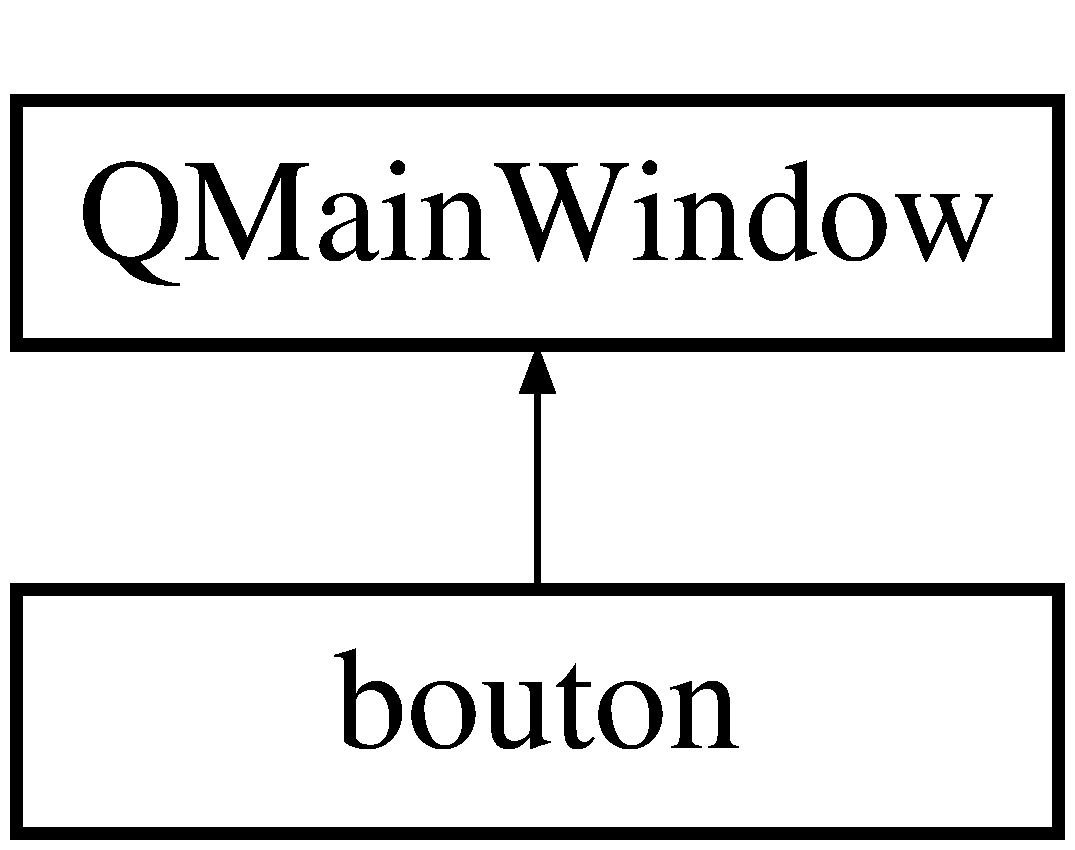
\includegraphics[height=2.000000cm]{classbouton}
\end{center}
\end{figure}


The documentation for this class was generated from the following files\+:\begin{DoxyCompactItemize}
\item 
bouton.\+h\item 
bouton.\+cpp\end{DoxyCompactItemize}

\hypertarget{classmanuel}{}\section{manuel Class Reference}
\label{classmanuel}\index{manuel@{manuel}}
Inheritance diagram for manuel\+:\begin{figure}[H]
\begin{center}
\leavevmode
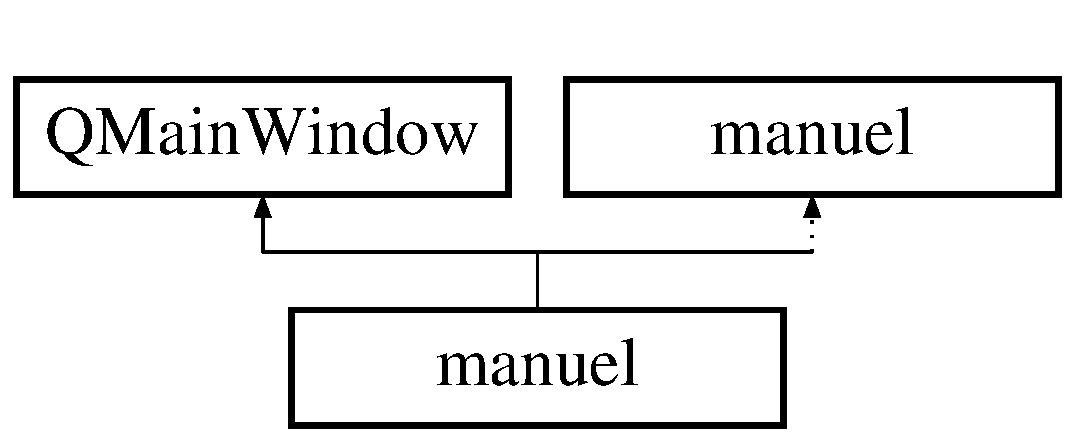
\includegraphics[height=2.000000cm]{classmanuel}
\end{center}
\end{figure}
\subsection*{Public Slots}
\begin{DoxyCompactItemize}
\item 
\hypertarget{classmanuel_a183a95b22521bfe735af3e2fbb4d9c6a}{}void {\bfseries on\+\_\+pbu\+Connect\+\_\+clicked} ()\label{classmanuel_a183a95b22521bfe735af3e2fbb4d9c6a}

\item 
\hypertarget{classmanuel_a67f7ff61f8a893ee477c3a212acf7a5b}{}void {\bfseries on\+\_\+pbu\+Read\+All\+\_\+clicked} ()\label{classmanuel_a67f7ff61f8a893ee477c3a212acf7a5b}

\item 
\hypertarget{classmanuel_a0f7554cdd82ddcd8343922ebdae44307}{}void {\bfseries on\+\_\+tab\+Widget\+\_\+current\+Changed} (int index)\label{classmanuel_a0f7554cdd82ddcd8343922ebdae44307}

\item 
\hypertarget{classmanuel_a4aa5f6166c22d218b9f5a208bb4d7ff3}{}void {\bfseries on\+\_\+tab\+Widget\+\_\+tab\+Close\+Requested} (int index)\label{classmanuel_a4aa5f6166c22d218b9f5a208bb4d7ff3}

\item 
\hypertarget{classmanuel_ab62cef62b9f9b30c8f92646ad643937b}{}void {\bfseries info} (const Q\+String \&source, const Q\+String \&message)\label{classmanuel_ab62cef62b9f9b30c8f92646ad643937b}

\item 
\hypertarget{classmanuel_a2549f1e2f5105bdb534483ef9908627a}{}void {\bfseries value\+Changed} (int table, const Q\+String \&name)\label{classmanuel_a2549f1e2f5105bdb534483ef9908627a}

\item 
\hypertarget{classmanuel_a601f4380110f989d7a2c56321af45bab}{}void {\bfseries Pince\+Ouverte} ()\label{classmanuel_a601f4380110f989d7a2c56321af45bab}

\item 
\hypertarget{classmanuel_ac5273c2bc152012426da7c821055e913}{}void {\bfseries Pince\+Ferme} ()\label{classmanuel_ac5273c2bc152012426da7c821055e913}

\item 
\hypertarget{classmanuel_a638a51cdd8db88e68b2c381f21d48a33}{}void {\bfseries Monter} ()\label{classmanuel_a638a51cdd8db88e68b2c381f21d48a33}

\item 
\hypertarget{classmanuel_af8478db2f4f3b6cec565c194242ae9e9}{}void {\bfseries Descendre} ()\label{classmanuel_af8478db2f4f3b6cec565c194242ae9e9}

\item 
\hypertarget{classmanuel_ac77a9f4a16274fde90f17d91e4d0200b}{}void {\bfseries Vers\+Palette} ()\label{classmanuel_ac77a9f4a16274fde90f17d91e4d0200b}

\item 
\hypertarget{classmanuel_aa0fb5a7b38ade3b5af97db12dd4b51d9}{}void {\bfseries Vers\+Table} ()\label{classmanuel_aa0fb5a7b38ade3b5af97db12dd4b51d9}

\item 
\hypertarget{classmanuel_a96c290b875cd9346b9d05fb4e4ef9f7b}{}void {\bfseries Moteur1} ()\label{classmanuel_a96c290b875cd9346b9d05fb4e4ef9f7b}

\item 
\hypertarget{classmanuel_aa2263d4038c638a2da7d13eceedfbfb2}{}void {\bfseries Moteur2} ()\label{classmanuel_aa2263d4038c638a2da7d13eceedfbfb2}

\item 
\hypertarget{classmanuel_a786dec81d83e52533e8336937bc07ea9}{}void {\bfseries Transfert\+Vers\+T2} ()\label{classmanuel_a786dec81d83e52533e8336937bc07ea9}

\item 
\hypertarget{classmanuel_ab0af857dd6d54c6b487d8bc171e239c1}{}void {\bfseries Transfert\+Vers\+T1} ()\label{classmanuel_ab0af857dd6d54c6b487d8bc171e239c1}

\item 
\hypertarget{classmanuel_a76c91d2d975ea63f8959f9ca64f3af3a}{}void {\bfseries Piece1} ()\label{classmanuel_a76c91d2d975ea63f8959f9ca64f3af3a}

\item 
\hypertarget{classmanuel_a8f4f5991c95c8143c008e29714ee79b8}{}void {\bfseries Piece2} ()\label{classmanuel_a8f4f5991c95c8143c008e29714ee79b8}

\item 
\hypertarget{classmanuel_a2e4eaf54e576a81402f52ac455920fa1}{}void {\bfseries Piece3} ()\label{classmanuel_a2e4eaf54e576a81402f52ac455920fa1}

\item 
\hypertarget{classmanuel_a3df76f297c72541be1b1d1e271fc16f0}{}void {\bfseries Piece4} ()\label{classmanuel_a3df76f297c72541be1b1d1e271fc16f0}

\item 
\hypertarget{classmanuel_a86c94ff88f2bcfcaa8c83db200c72671}{}void {\bfseries Piece5} ()\label{classmanuel_a86c94ff88f2bcfcaa8c83db200c72671}

\item 
\hypertarget{classmanuel_ae82822e597050c3c0d5d250444ad2570}{}void {\bfseries Piece6} ()\label{classmanuel_ae82822e597050c3c0d5d250444ad2570}

\item 
\hypertarget{classmanuel_a641b749491435729df92ecf2465ac42a}{}void {\bfseries Piece7} ()\label{classmanuel_a641b749491435729df92ecf2465ac42a}

\item 
\hypertarget{classmanuel_a3c040bde59499ba0c6d12a8760a6d02c}{}void {\bfseries Piece8} ()\label{classmanuel_a3c040bde59499ba0c6d12a8760a6d02c}

\item 
\hypertarget{classmanuel_a5e9e6950d1e7fd6177540f1fcc9a15d3}{}void {\bfseries Piece9} ()\label{classmanuel_a5e9e6950d1e7fd6177540f1fcc9a15d3}

\item 
\hypertarget{classmanuel_ad749b87bd8f2dba5ae7ea0a9cafe51ea}{}void {\bfseries Piece10} ()\label{classmanuel_ad749b87bd8f2dba5ae7ea0a9cafe51ea}

\item 
\hypertarget{classmanuel_ac63ea0e5e2255597ddca5f09d3fd8fc2}{}void {\bfseries Piece11} ()\label{classmanuel_ac63ea0e5e2255597ddca5f09d3fd8fc2}

\item 
\hypertarget{classmanuel_ae1f84003d37fea305651a7b69fd61b30}{}void {\bfseries Piece12} ()\label{classmanuel_ae1f84003d37fea305651a7b69fd61b30}

\item 
\hypertarget{classmanuel_a6d7deeb5ac2b64974c35f83254f2d379}{}void {\bfseries Piece13} ()\label{classmanuel_a6d7deeb5ac2b64974c35f83254f2d379}

\item 
\hypertarget{classmanuel_a21e5f29a533c78a519570e2bcf347ade}{}void {\bfseries Piece14} ()\label{classmanuel_a21e5f29a533c78a519570e2bcf347ade}

\item 
\hypertarget{classmanuel_a47857054f569ede453cb1fc1d6e73042}{}void {\bfseries Piece15} ()\label{classmanuel_a47857054f569ede453cb1fc1d6e73042}

\item 
\hypertarget{classmanuel_ab87e9fdbab41d5f67c5ddebce8cf765a}{}void {\bfseries Piece16} ()\label{classmanuel_ab87e9fdbab41d5f67c5ddebce8cf765a}

\item 
\hypertarget{classmanuel_a37b2bdd5ff18aab7ee112656feed3ac3}{}void {\bfseries Piece17} ()\label{classmanuel_a37b2bdd5ff18aab7ee112656feed3ac3}

\item 
\hypertarget{classmanuel_a1311544612c1ee38eb55d198c728caf6}{}void {\bfseries Piece18} ()\label{classmanuel_a1311544612c1ee38eb55d198c728caf6}

\item 
\hypertarget{classmanuel_a415fa6ffa8e742dc96dfbff7b09fabda}{}void {\bfseries Piece19} ()\label{classmanuel_a415fa6ffa8e742dc96dfbff7b09fabda}

\item 
\hypertarget{classmanuel_a153ee419c015f0e738d5c28592bbc2a3}{}void {\bfseries Piece20} ()\label{classmanuel_a153ee419c015f0e738d5c28592bbc2a3}

\item 
\hypertarget{classmanuel_a21d99614b897025bde678a43d116c9ea}{}void {\bfseries Bute\+A} (int state)\label{classmanuel_a21d99614b897025bde678a43d116c9ea}

\item 
\hypertarget{classmanuel_a3c32d0f15b8d23a0d97db3c8eb9f5eae}{}void {\bfseries Bute\+V} (int state)\label{classmanuel_a3c32d0f15b8d23a0d97db3c8eb9f5eae}

\item 
\hypertarget{classmanuel_a1814206c6a6774cfd9546a60e38716e0}{}void {\bfseries Bute\+S} (int state)\label{classmanuel_a1814206c6a6774cfd9546a60e38716e0}

\item 
\hypertarget{classmanuel_a22e7d533de06672e422204b4743e1251}{}void {\bfseries Bute\+Att} (int state)\label{classmanuel_a22e7d533de06672e422204b4743e1251}

\item 
\hypertarget{classmanuel_a96fcc81ea011522b162ea0735e5152cb}{}void {\bfseries Reset} ()\label{classmanuel_a96fcc81ea011522b162ea0735e5152cb}

\item 
\hypertarget{classmanuel_ada44cd143e8fe0dec076ae8dc719ec14}{}void {\bfseries Auto} ()\label{classmanuel_ada44cd143e8fe0dec076ae8dc719ec14}

\item 
\hypertarget{classmanuel_aff5e70155acb9426ad7c9b6b11556cc9}{}void {\bfseries Pom} ()\label{classmanuel_aff5e70155acb9426ad7c9b6b11556cc9}

\end{DoxyCompactItemize}
\subsection*{Public Member Functions}
\begin{DoxyCompactItemize}
\item 
\hypertarget{classmanuel_a31a13d8ea56748784c55821c3e09ba23}{}{\bfseries manuel} (Q\+Widget $\ast$parent=0)\label{classmanuel_a31a13d8ea56748784c55821c3e09ba23}

\end{DoxyCompactItemize}
\subsection*{Protected Member Functions}
\begin{DoxyCompactItemize}
\item 
\hypertarget{classmanuel_a3d72b69379f3e8cac58912b53bb0ddec}{}void {\bfseries close\+Event} (Q\+Close\+Event $\ast$event)\label{classmanuel_a3d72b69379f3e8cac58912b53bb0ddec}

\end{DoxyCompactItemize}


The documentation for this class was generated from the following files\+:\begin{DoxyCompactItemize}
\item 
manuel.\+h\item 
bouton.\+cpp\item 
manuel.\+cpp\end{DoxyCompactItemize}

%--- End generated contents ---

% Index
\backmatter
\newpage
\phantomsection
\clearemptydoublepage
\addcontentsline{toc}{chapter}{Index}
\printindex

\end{document}
